

\chapter{Modelling of a rotating free-floating object dynamic interactions with a mass moving on its surface}
\label{ch:Stability study}

\section{Introduction: What Proof of Concept}
\label{Introduction: What Proof of Concept}
In this chapter is designing mass changes as control method one needs to establish the effect of changes of mass distributioon on a rotating free floating rotational motion and determine if there are and if so under what kind of conditions the motion of a mass at the surface of a free floating objects will imact its rotational motions
delpoyment of structure on frre floating object

define the stability of the rotational motion of the obejct???

System definition and model: The system is composed of an undeformable rotating object and a modular robot made out of identical spherical modules. The robots moves and deploys itself at the surface of the object by maintianing contact at all time. As the rotational motion is the only focus of this study, the system is considered to be isolated.
The best way to model is to use 

Write..\gls{ghc}
Write..\gls{ghc}.

\section{Illustration of the approach: the Yo-Yo despin mechanism}
\label{Illustration of the approach: the Yo-Yo despin mechanism}
\subsection{Yo-Yo despin mechanism description}
\label{Yo-Yo despin mechanism description}
\begin{figure}[h]
	\begin{center}
		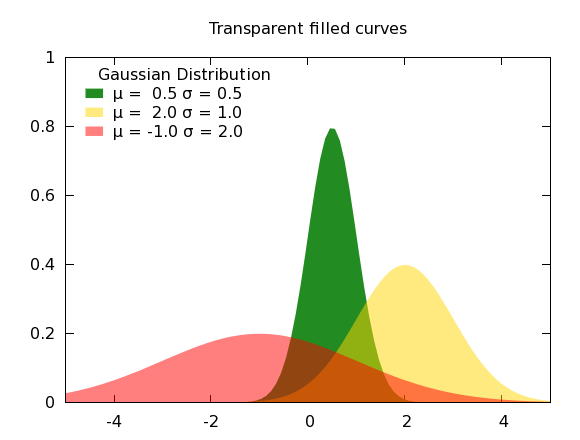
\includegraphics [width=12cm]{Figures/Background/pic.png}
		\caption{Figure Caption.}
		\label{fig:Yo-Yo despin mechanism seen in its plane of rotation}
	\end{center}
\end{figure} 



\section{System modelling}
\label{System modelling}
The Yo-Yo despin mechanism is discrete in order to generalise the robot and object were considered as a deformablee continuum where a rigid part (the object) would interact with a deformable part (the robot). The general model can be discrtized in order to accomodate the modular structure of the robot and simplify the dynamic equations of the system.

the model is directly derived from [PAPER]
\subsection{Continuous model}
\label{Continuous model}
\subsection{Discrete point mass model}
\label{Discrete point mass model}

Write.. \gls{pe}.

Write.. \glspl{pe}.

\section{Hamiltonian Lagrange formulation}
\label{Hamiltonian Lagrange formulation}

Write.. \gls{pe}.

Write.. \glspl{pe}.

%\begin{figure}[h]
% \begin{center}
% 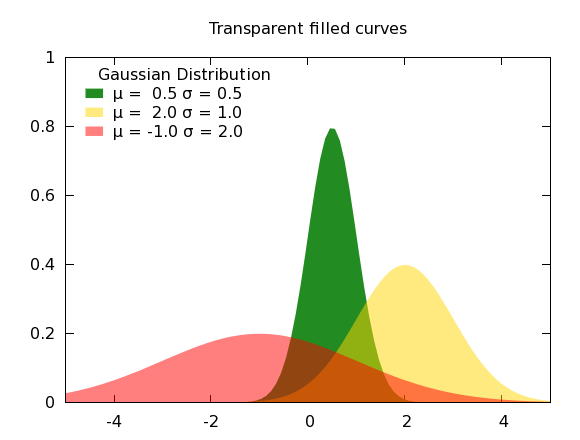
\includegraphics [width=12cm]{Figures/Background/pic.png}
% \caption{Figure Caption.}
% \label{fig:label}
%\end{center}
%\end{figure} 
%
%\cite{gum, ghc-smp}
%
%\subsection{Subsection}
%
%\begin{table}[h]
%\begin{center}
%\begin{tabular}{c c c c} % centered columns (4 columns)
%\hline\hline %inserts double horizontal lines
%Case & Method\#1 & Method\#2 & Method\#3 \\ [0.5ex] % inserts table 
%%heading
%\hline % inserts single horizontal line
%1 & 50 & 837 & 970 \\ % inserting body of the table
%2 & 47 & 877 & 230 \\
%3 & 31 & 25 & 415 \\
%4 & 35 & 144 & 2356 \\
%5 & 45 & 300 & 556 \\ [1ex] % [1ex] adds vertical space
%\hline %inserts single line
%\end{tabular}\caption{Table Caption}
%\label{tab:lable}
%\end{center}
%\end{table}
%
%
%\subsubsection{Subsubsection}